\section{Kompilierung und Programmierung}\label{section:konzeption:kompilierung-und-programmierung}

Nach \autoref{requirement:Kompilierung} soll die Kompilierung der Programme von Nutzern innerhalb der IDE ermöglicht werden. Laut Unteranforderung (a) soll daher ein CrossLab-Service für die Bereitstellung und Nutzung von Compilern entwickelt werden. Diese sollen nach Unteranforderung (b) von der IDE für die Nutzung von Compilern verwendet werden. Weiterhin soll nach \autoref{requirement:Programmierung von Steuereinheiten} die Programmierung von Steuereinheiten innerhalb der IDE ermöglicht werden. Laut Unteranforderung (a) soll daher ein CrossLab-Service für die Programmierung von Steuereinheiten entwickelt werden. Dieser soll nach Unteranforderung (b) von der IDE für die Programmierung von Steuereinheiten verwendet werden. Dementsprechend werden im Folgenden der \textit{Compilation Service} sowie der \textit{Programming Service} vorgestellt.

Der Compilation Service Consumer besitzt nur eine Funktion, die es ermöglicht, die Kompilierung eines Ordners anzufragen. Dabei können zusätzliche Optionen für den Compiler sowie das gewünschte Format der Ausgabe angegeben werden. Die möglichen Ausgabeformate können auf der Seite des Compilation Service Producer über entsprechende Schemata definiert und hinzugefügt werden. Die registrierten Ausgabeformate können dann in der Servicebeschreibung des Compilation Service Producer hinterlegt werden. Während der Erstellung eines Experiments kann das gewünschte Ausgabeformat für die Verbindung eines Compilation Service Consumer und eines Compilation Service Producer in der Verbindungskonfiguration angegeben werden. Die Behandlung von Kompilieranfragen ist abhängig vom verwendeten Compiler. Bei einer erfolgreichen Kompilierung wird das Ergebnis in dem festgelegten Ausgabeformat zusammen mit den Meldungen des Compilers an den Compilation Service Consumer gesendet. Falls die Kompilierung fehlschlägt, werden nur die Fehlermeldungen des Compilers versendet.

Der Programming Service Consumer besitzt nur eine Funktion, die es ermöglicht, eine Programmieranfrage zu starten. Diese muss entweder eine Datei, z.B. das Ergebnis einer Kompilierung, oder einen Ordner mit dem entsprechenden Programm enthalten. Dabei könnte der Programming Service Producer über seine Servicebeschreibung angeben, welche Formate unterstützt werden. Beim Erhalt einer Programmieranfrage soll der Programming Service Producer die Programmierung der Steuereinheit starten. Sobald die Programmierung abgeschlossen wurde wird eine Antwort an den Programming Service Consumer gesendet.

Die betrachtete Experimentkonfiguration wird zunächst um ein weiteres Laborgerät erweitert. Dieses stellt einen Compiler über einen entsprechenden Compilation Service Producer bereit. Die IDE wird um einen Compilation Service Consumer sowie einen Programming Service Consumer erweitert. Die Steuereinheit wird um einen Programming Service Producer erweitert. Die IDE wird dann über die neu hinzugefügten CrossLab-Services mit dem Compiler und der Steuereinheit verbunden. Die Erweiterung der betrachteten Experimentkonfiguration ist in \autoref{figure:experimentkonfiguration:kompilierung} dargestellt.

\begin{figure}[tbp]
    \centering
    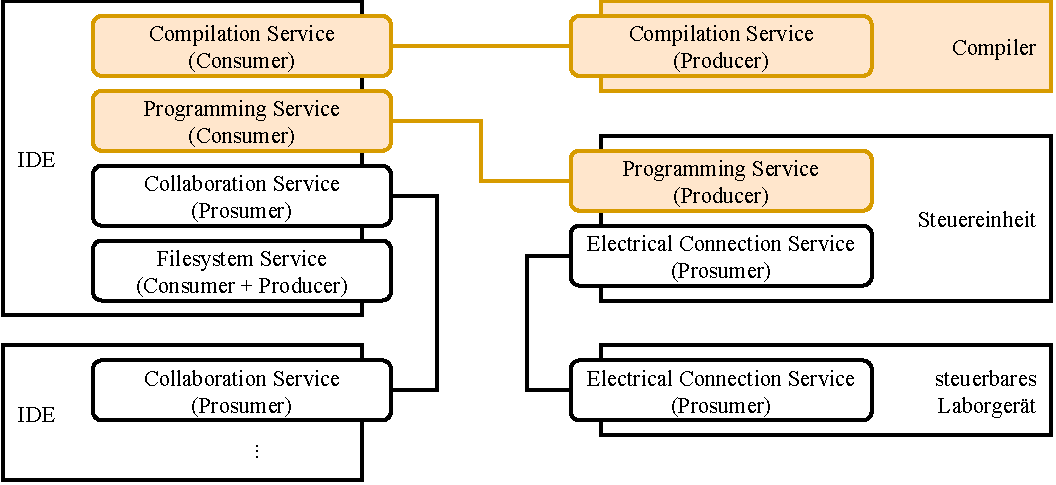
\includegraphics[width=\textwidth]{diagrams/experimentkonfigurationen/Experimentkonfiguration-03.drawio.pdf}
    \caption{Experimentkonfiguration (+ Kompilierung \& Programmierung)}
    \label{figure:experimentkonfiguration:kompilierung}
\end{figure}